\chapter{Exploración}

Para los problemas de grafos ser capaz de recorrer los vértices del grafo en búsqueda de información nos ofrece muchas herramientas para estos problemas.  

Para esto recordemos las búsquedas que vimos en el capítulo 2, la búsqueda exhaustiva, DFS y BFS; ya que los recorridos básicos de un grafo son estos mismos.

El primer recorrido que veremos es la DFS, recordemos un poco acerca de como se comporta.

\chapter{DFS}

La DFS o búsqueda en profundidad es una técnica que explora un grafo vértice por vértice. Útil para encontrar vértices alcanzables y hacer coloreo. 

Iniciando en un primer nodo, en cada paso busca un vecino del nodo actual y lo explora, si no encuentra un vértice sin explorar, regresa por el camino que tomo en búsqueda de vértices que se haya dejado.


\begin{center}
	DIBUJO TODO
\end{center}


\pagebreak

Y el código de una DFS es igual al que ya habíamos visto previamente.

\begin{lstlisting}
	vector<int> adyacencia[100050];
	bool visitado[100050];
	void DFS(int vertice) {
		visitado[vertice]=true;
		for (int i=0; i < adyacencia[vertice].size(); i++) {
			int vecino = adyacencia[vertice][i];
			if (!visitado[vecino]) {
				DFS(vecino);
			}
		}
	}
\end{lstlisting}

\section*{Ejemplo: Conectividad}

Pedro vive en un pequeño país de Oceanía, formado por \(N\) islas enumeradas del \(1\) al \(N\). Entre estas islas hay \(M\) túneles submarinos que las conectan, permitiendo manejar un coche de isla a isla. 

Pedro quiere saber si puede tomar su coche de la isla \(a\) a la isla \(b\).

\textbf{Entrada}\\
En la primera línea tendrás cuatro enteros \(N\), \(M\), \(a\) y \(b\) --- El número de islas en el país, el número de túneles, la isla donde Pedro está y la isla a donde quiere ir.

En cada una de las siguientes \(M\) líneas vendrá la descripción de un túnel, cada túnel esta descrito por dos enteros \(u\) y \(v\) indicando que el túnel conecta la isla \(u\) con la \(v\).

\textbf{Salida}\\
Imprime \texttt{SI} si es posible viajar de la isla \(a\) a la isla \(b\) en coche. Si es imposible imprime \texttt{NO}.

\textbf{Ejemplo}\\
\begin{casebox3}
	\ecase{
		6 5 1 6\\
		1 2\\		
		4 6\\
		2 3\\
		3 1\\
		3 4
	}{SI}{
		Toma el siguiente camino\\
		\(1\rightarrow3\rightarrow4\rightarrow6\)
	}
	\ecase{
	6 5 1 6\\
	1 2\\		
	2 3\\
	1 3\\
	4 5\\
	5 6
	}{NO}{
	Es imposible viajar de 1  a 6\\
	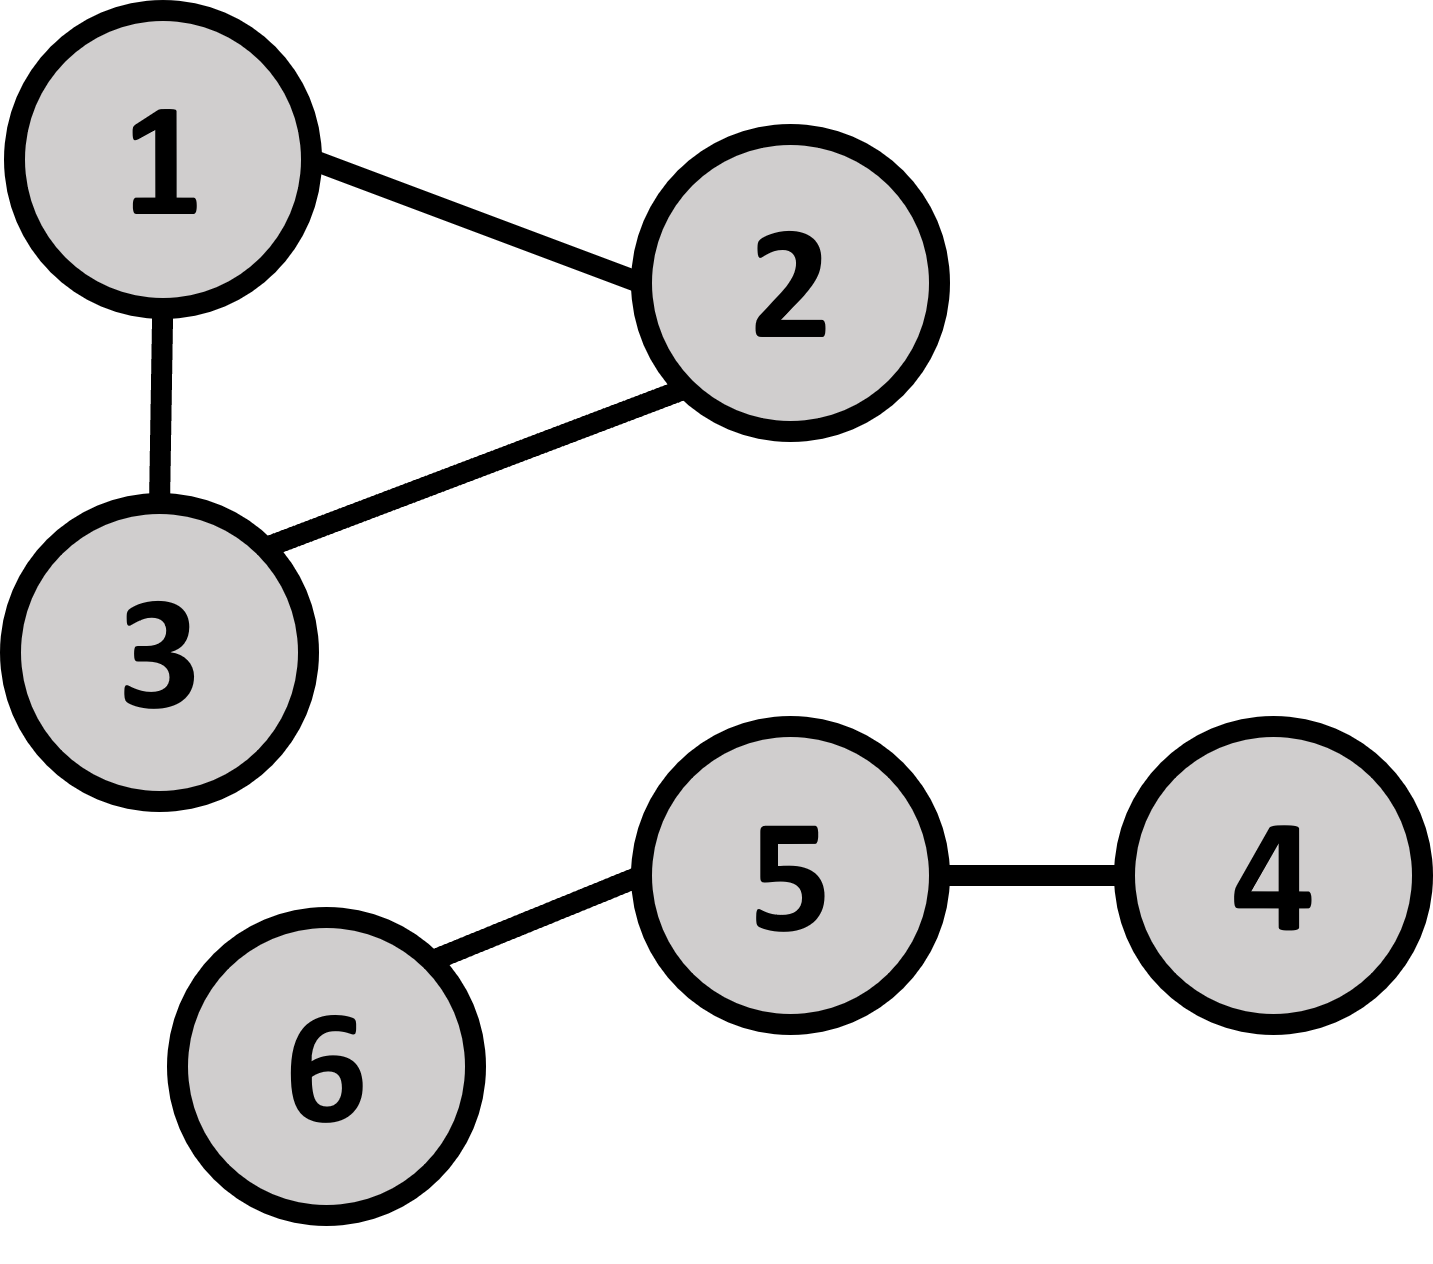
\includegraphics[scale=0.2]{grafos/islas2}
	}
\end{casebox3}

\textbf{Límites}
\begin{plimits}
	\item \(1 \leq N \leq 10^5\)
	\item \(1 \leq M \leq 2\times10^5\)
\end{plimits}

Fuente: TODO

\subsection*{Solución} 

Si descubrimos todos los vértices que se pueden alcanzar usando túneles desde \(a\), podremos saber si entre ellos esta \(b\) o no. Para esto usamos una DFS.

La idea principal es crear una DFS que regrese verdadero si puede encontrar un vértice y falso si no puede, para esto haremos que la DFS que creemos sea una función booleana que regrese la respuesta.

\begin{minipage}{\linewidth}
\begin{lstlisting}
bool buscarB(int actual, int b) {
	if (actual==b)return true;
	visitado[actual] = true;
	for (int vecino: adyacencia[actual]) {
		if (visitado[vecino] == false) {
			visitado[vecino]=true;
			if (buscarB(vecino, b)) {
				return true;
			}
		}
	}
	return false;
}

[...]

if (buscarB(a, b)) {
	cout << "SI";
} else {
	cout << "NO";
}
\end{lstlisting}
\end{minipage}

\section{Complejidad}
La complejidad de una DFS es fácil de calcular, basta con ver que cada vértice es a los más explorado una única vez; mientras que cada arista es visitada a los más dos veces, una por cada vértice que conecta.

Entonces, la complejidad total de la DFS es \(O(V+E)\). Donde \(V\) es el número de vértices y \(E\) la cantidad de aristas.

\section{Problemas clásicos}
A continuación veremos problemas clásicos de DFS, lo que querremos es que primero leas e intentes resolver los problemas. Evita leer la solución hasta haberlo intentado y se hayan acabado las ideas.

\subsection{Coloreando componentes}
Armando le gusta colorear, esta vez encontró un libro que muestra constelaciones.
El libro ilustra \(N\) estrellas conectadas con \(M\) líneas. Las estrellas están enumeradas de \(1\) a \(N\).

Una constelación es un grupo de estrellas que están conectadas entre ellas, por ejemplo la siguiente imagen muestra tres constelaciones:

\begin{center}
	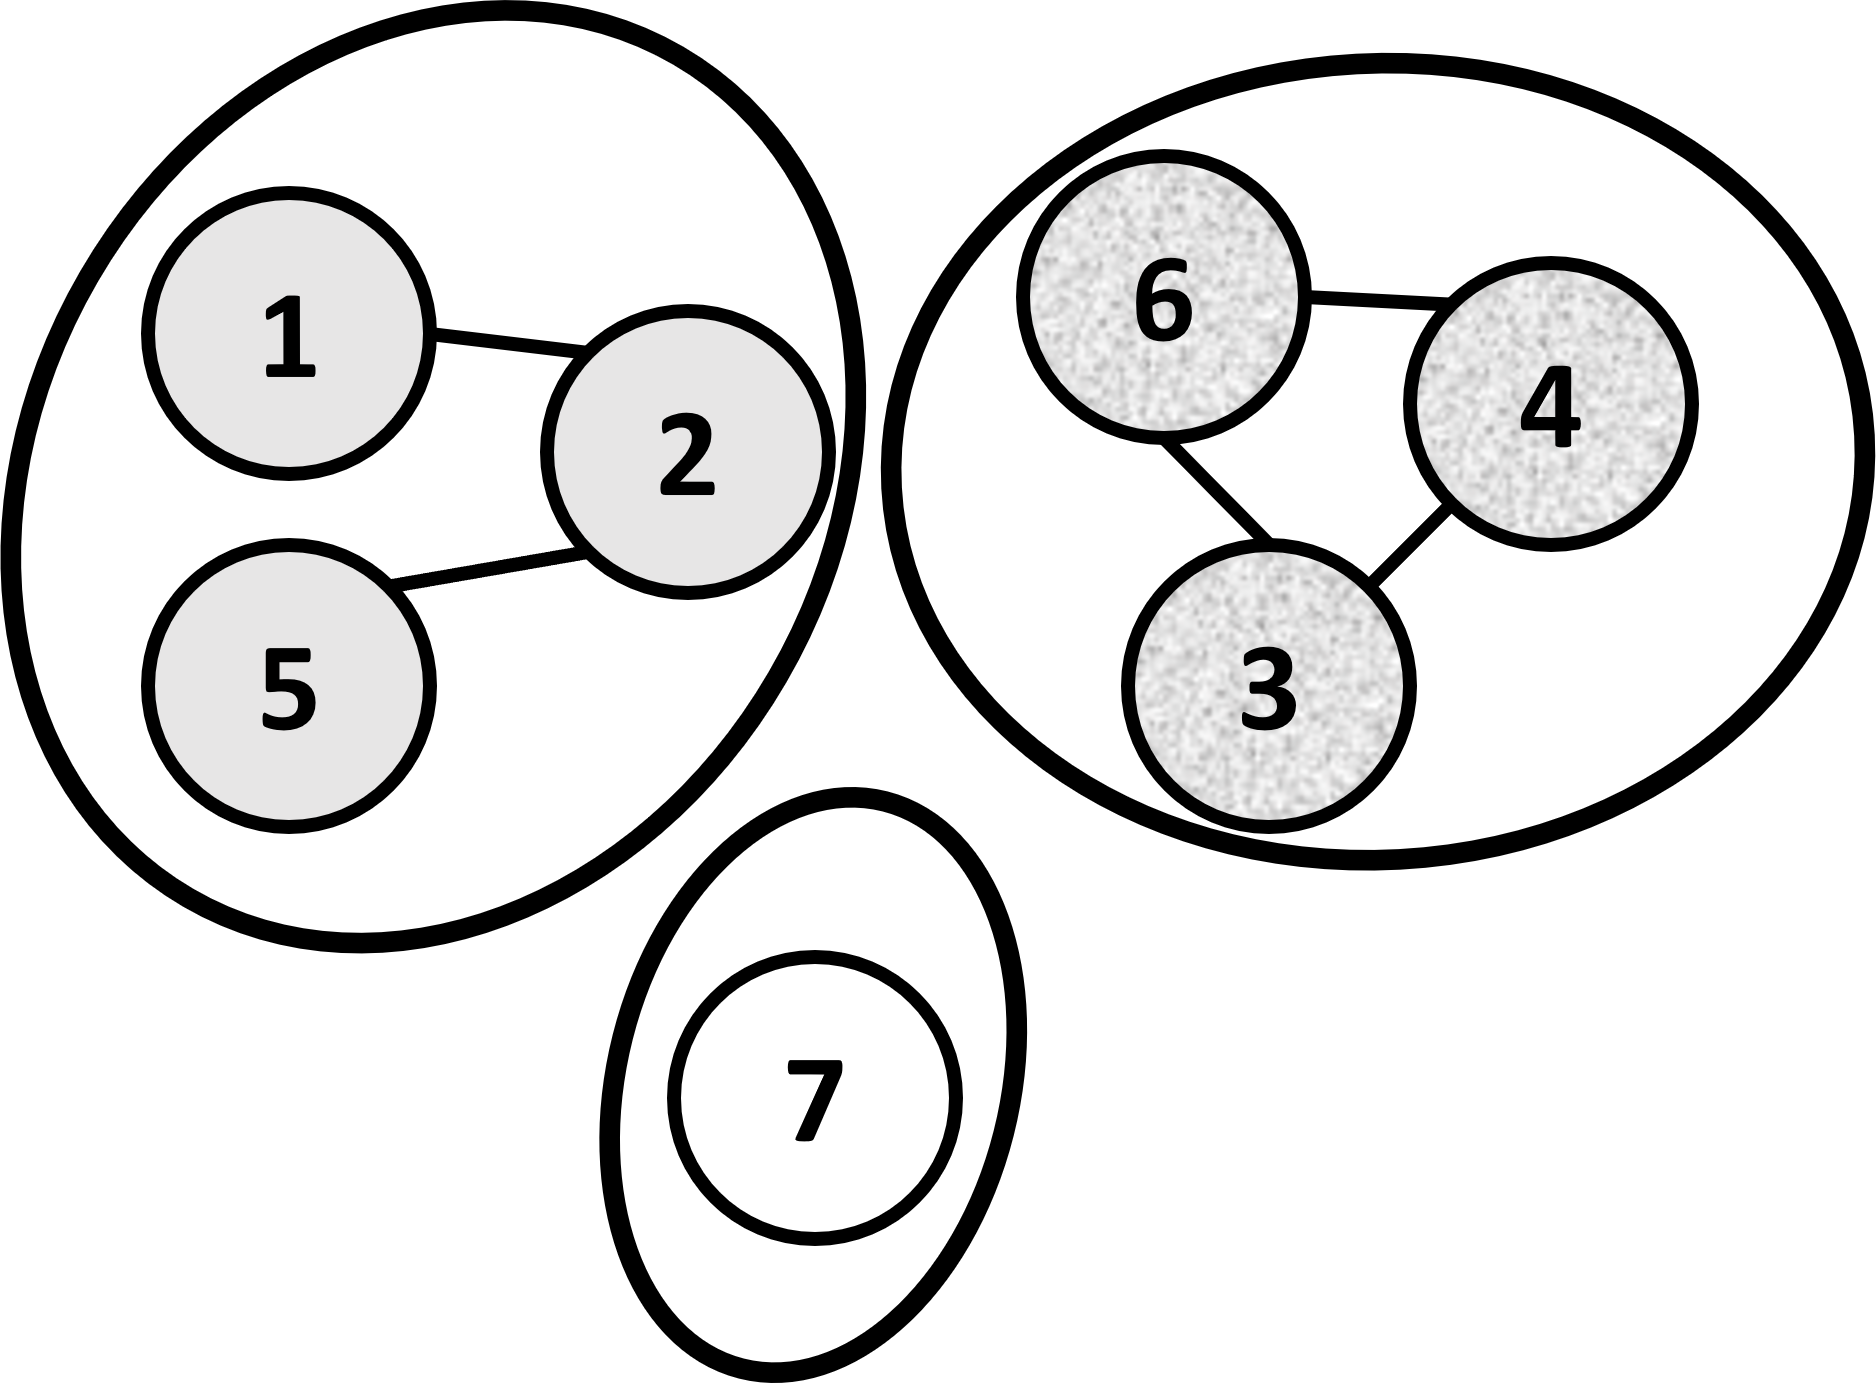
\includegraphics[scale=0.3]{grafos/constelaciones}
\end{center}

Armando quiere colorear las estrellas de forma que si dos estrellas son de la misma constelación tengan el mismo color, pero sean coloreadas diferentes si son de distintas constelaciones. Para esto el dispone de \(N\) colores enumerados \(1, 2, 3, \ldots, N\).

Dado la descripción del libro, determina el color de cada estrella que cumpla las reglas de Armando.

\textbf{Entrada}\\
La primeras dos líneas tendrán dos enteros \(N\) y \(M\) --- La cantidad de estrellas y el número de conexiones.

En las siguientes \(M\) líneas vendrán las conexiones, cada conexión será descrita por dos enteros, el número de estrellas que conecta.

\textbf{Salida}\\
Imprime \(N\) enteros, el \(i\)-ésimo entero será el color de la estrella \(i\).

Cualquier coloración válida será aceptada.

\textbf{Ejemplo}\\
\begin{casebox3}
	\ecase{
		7 5\\
		6 4\\
		4 3\\
		3 6\\
		2 5\\
		1 2
	}{1 1 2 2 1 2 3}{La imagen de ejemplo.}
\end{casebox3}

\textbf{Límites}\\
\(1\leq N \leq 10^5\)\\
\(1\leq M \leq 2\times 10^5\)

Enlace TODO:

\pagebreak

\subsubsection*{Pista}
Una pista para resolverlo es que un problema puede requerir de varias DFS.


\subsubsection*{Solución}
Una observación importante es que una constelación es un grupo de estrellas conectados ya sea de forma directa o indirecta. Este hecho significa que si iniciamos una DFS en una estrella, visitaremos todos las estrellas de la constelación.

Entonces, lo que podemos hacer es iniciar una DFS por cada constelación e ir coloreando las estrellas que vayamos visitando con un color especificado. 

Para esto, lo que haremos es un ciclo que vaya por todas las estrellas, cada que encuentre una estrella sin color, creamos una DFS que colorea su constelación.

\begin{lstlisting}
int color=0;
for (int i =0; i < N; i++) {
	if (coloreado[i]==0) {
		color++;
		dfs(i, color);
	}
}
\end{lstlisting}

\subsection{Componentes conexos}

Las constelaciones en el ejemplo anterior reciben el nombre de componente conexa, en el caso ejemplo teníamos tres componentes conexas. Entonces, una componente conexa es un conjunto de vértices más grande posible para el cual es posible viajar de uno a cualquier otro usando las aristas.

Un grafo es conexo si se puede viajar de cualquier vértice a cualquier otro usando las aristas, es decir, solo hay un componente conexo que incluye a todos los vértices.

La DFS resplandece en problemas de conectividad como lo fueron los ejemplos anteriores.

\subsection{Bipartito}
Llamamos bipartito a un grafo si se puedes separar los vértices en dos grupos de forma de que cada vértice pertenezca a exactamente un grupo y las aristas solo conecten vértices de grupos contrarios.

Por ejemplo, el siguiente grafo es bipartito:

\begin{center}
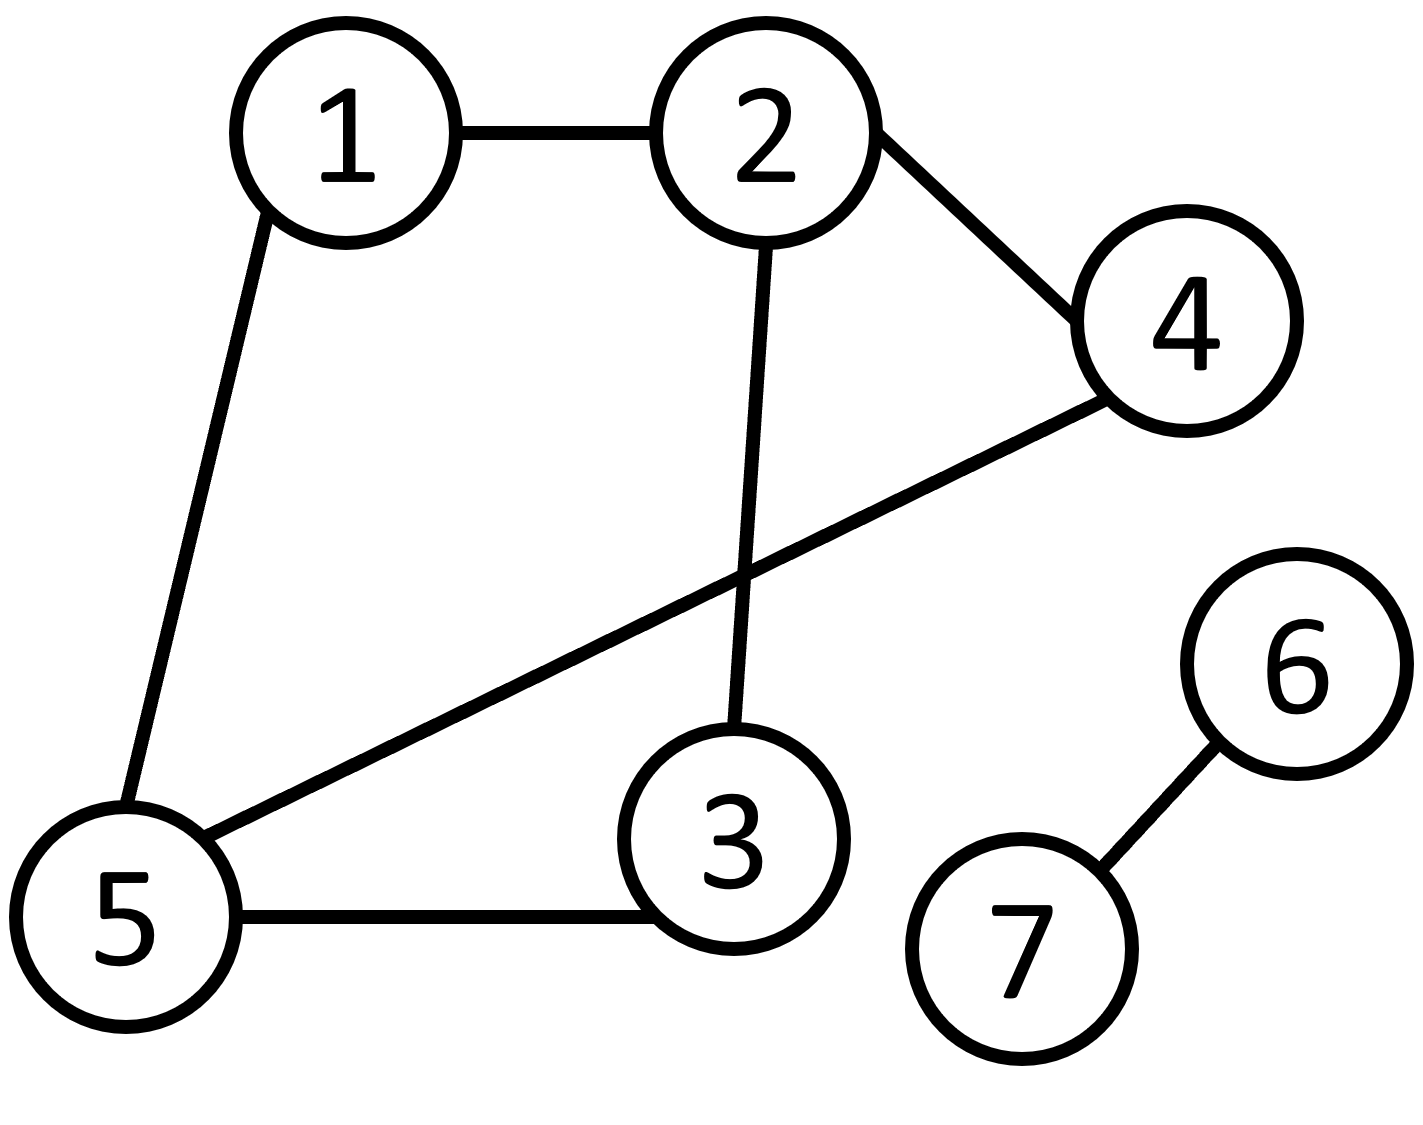
\includegraphics[scale=0.25]{grafos/bipartitoA}
\end{center}

Porque se puede separar en dos grupos \(\{2, 5, 7\}\) y \(\{1, 4, 3, 6\}\):	

\begin{center}
	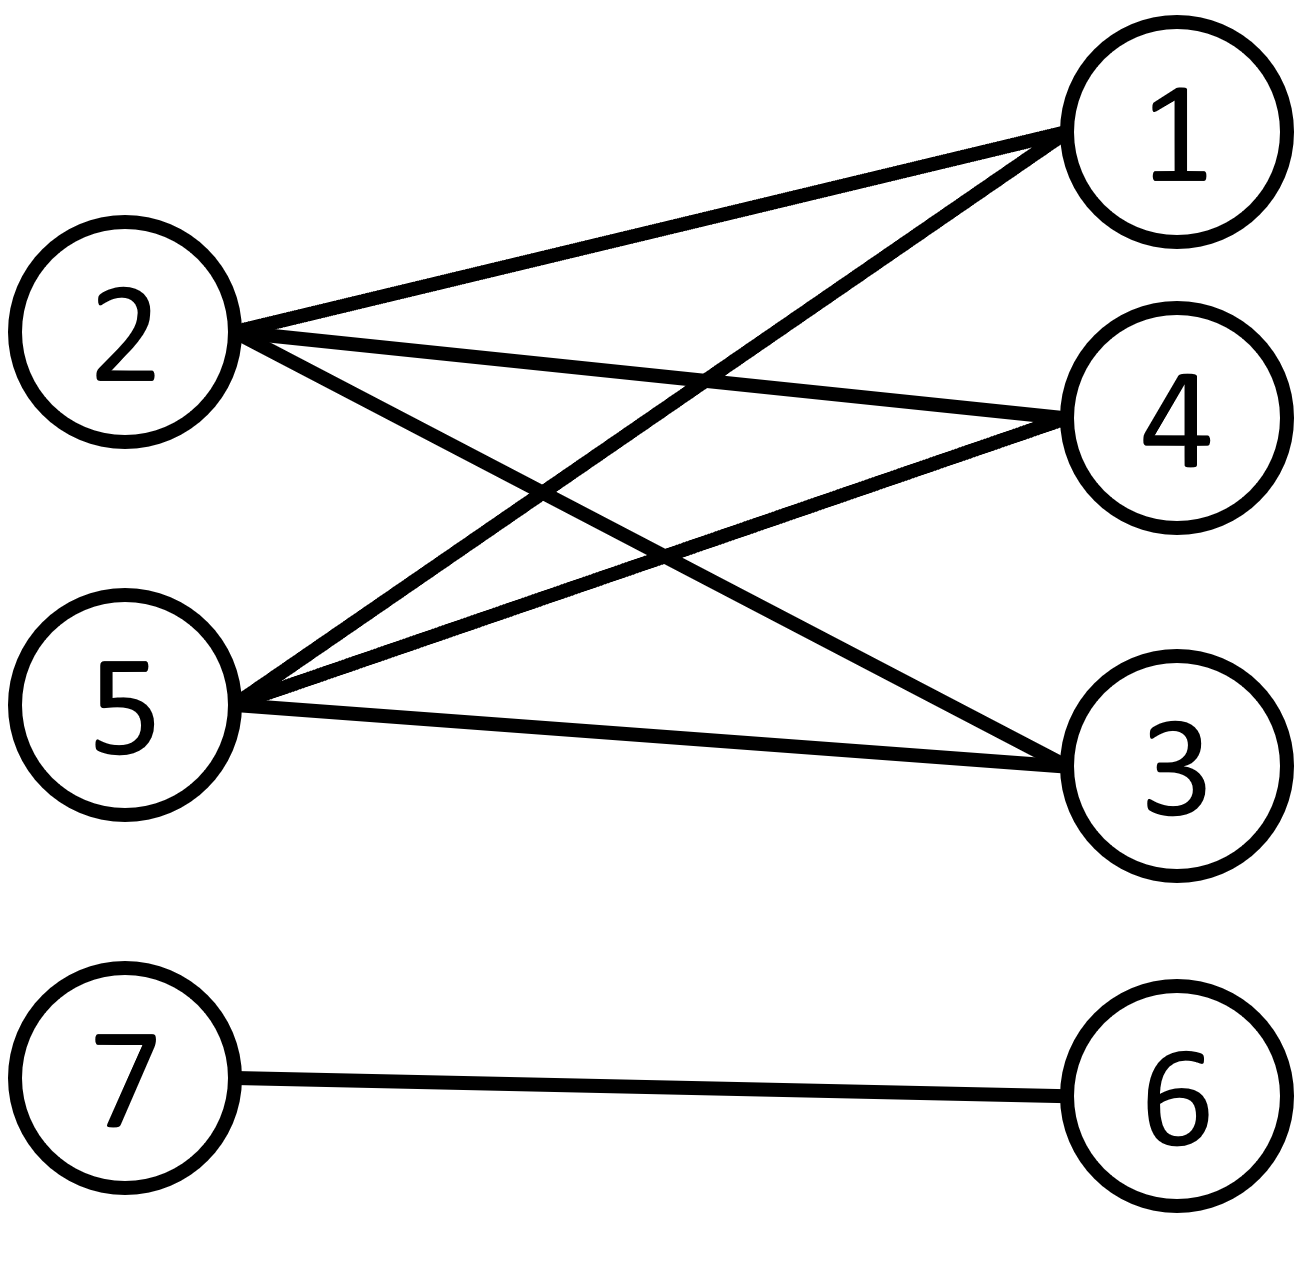
\includegraphics[scale=0.25]{grafos/bipartitoB}
\end{center}

Mientras que un grafo como el siguiente no es bipartito, no se puede separar en dos grupos con todas las aristas entre los dos grupos:

\begin{center}
	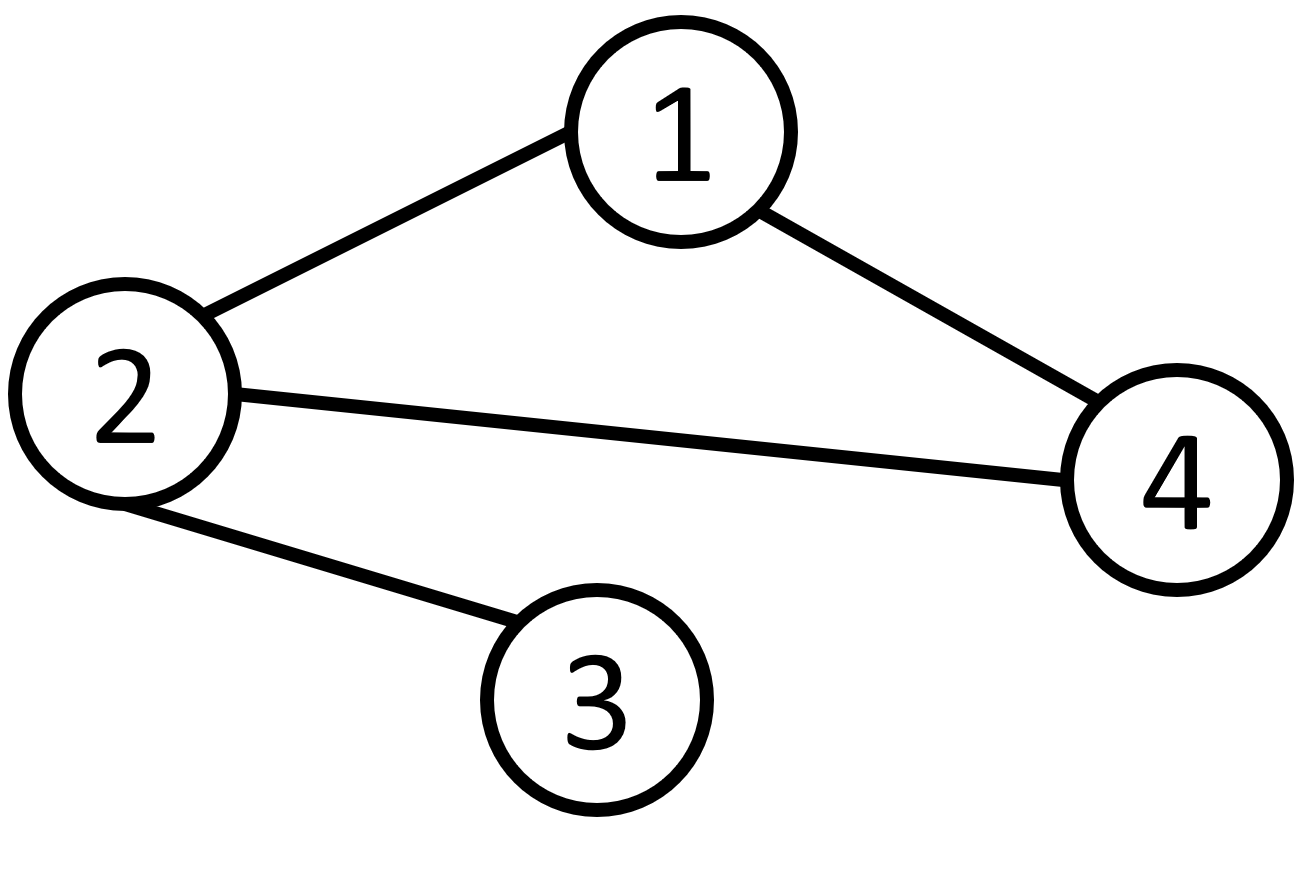
\includegraphics[scale=0.25]{grafos/nobip}
\end{center}

Dado un grafo determina si es bipartito o no.

\textbf{Entrada}\\
En la primera línea habrá dos enteros \(V\) y \(E\) --- La cantidad de vértices y aristas.

En las siguientes \(E\) líneas vendrán la descripción de las aristas.

\textbf{Salida}\\
Imprime \verb|SI| cuando el grafo sea bipartito, imprime \verb|NO| en caso contrario.

\textbf{Ejemplo}\\
\begin{casebox2}
	\scase{
		7 7\\
		1 2\\
		2 4\\
		2 3\\
		1 5\\
		5 3\\
		4 5\\
		6 7
	}{
	SI
	}
	\scase{
		4 4\\
		1 2\\
		2 4\\
		4 1\\
		2 3
	}{
	NO
	}
\end{casebox2}

\textbf{Límites}\\
\(1\leq N \leq 10^5\)\\
\(1\leq M \leq 4\times10^5\)
	

\pagebreak

\subsubsection*{Pista}
La solución sigue una idea similar al problema anterior.

\subsubsection*{Solución}
Podemos hacer una DFS que coloree el grafo con dos colores, digamos blanco y negro. 

Haremos que la DFS coloree el grafo de forma alternada tal que cada arista conecte un vértice blanco con un vértice negro. 

Evidentemente esto es lo mismo que separar los vértices en los dos grupos del grafo bipartito. Si se puede hacer esta coloración, entonces el grafo es bipartito, caso contrario no lo es.

Para esto haremos que la DFS coloree cada vértice que explore, tal que cada que se mueva una arista, alterne el color. Si en algún momento encuentras una contradicción, dos colores iguales juntos, entonces el grafo no es bipartito.


Crearemos una DFS recursiva que regrese verdadero si se puede hacer la coloración y falso en caso contrario. La DFS tiene como argumentos en cual vértice se encuentra y de que color debe ser el vértice. Alternamos el color cada que llamamos la DFS en un vecino y revisamos que en ningún momento tengamos un vecino con el mismo color.

\begin{minipage}{\linewidth}
\begin{lstlisting}
int coloreado[100050];
bool DFS(int vertice, int color) {
	int otroColor=1;
	if (color==1)
		otroColor=2;
	for (int vecino: adyacencia[vertice]) {
		if (coloreado[vecino]==0) {
			if (!DFS(vecino, otroColor)) {
				return false;
		} else if (coloreado[vecino]==color) {
			return false;
		}
	}
	return true;
}

int main() {
	[...]
	for (int i =0;i < N;i++) {
		if (coloreado[i]==0) {
			if (!DFS(i, 1)) {
				cout << "NO";
				return 0;
			}
		}
	}
	cout << "SI";
	return 0;
}
\end{lstlisting}
\end{minipage}